\hypertarget{barcode_8inc}{
\section{barcode.inc File Reference}
\label{barcode_8inc}\index{barcode.inc@{barcode.inc}}
}
\subsection*{Functions}
\begin{CompactItemize}
\item 
\hyperlink{barcode_8inc_6d3645af0ef526e4f64d28dcbdceb74f}{checkBarcode} (\$barcode)
\item 
\hyperlink{barcode_8inc_e10c37e4f9f9b7c6617a388351a27c99}{getBarcodeInfo} (\$barcode)
\end{CompactItemize}


\subsection{Detailed Description}
Functions for the handling of different barcodes 

Definition in file \hyperlink{barcode_8inc-source}{barcode.inc}.

\subsection{Function Documentation}
\hypertarget{barcode_8inc_6d3645af0ef526e4f64d28dcbdceb74f}{
\index{barcode.inc@{barcode.inc}!checkBarcode@{checkBarcode}}
\index{checkBarcode@{checkBarcode}!barcode.inc@{barcode.inc}}
\subsubsection{\setlength{\rightskip}{0pt plus 5cm}checkBarcode (\$ {\em barcode})}}
\label{barcode_8inc_6d3645af0ef526e4f64d28dcbdceb74f}


Checks to see if a valid, handalable, barcode was entered. \begin{Desc}
\item[Parameters:]
\begin{description}
\item[{\em \$barcode}]The Barcode to be checked \end{description}
\end{Desc}
\begin{Desc}
\item[Returns:]The type of barcode entered if valid, FALSE if it is not \end{Desc}


Array containinf info on the given UPC 

Definition at line 11 of file barcode.inc.

References XMLRPC\_\-prepare(), and XMLRPC\_\-request().

Here is the call graph for this function:\nopagebreak
\begin{figure}[H]
\begin{center}
\leavevmode
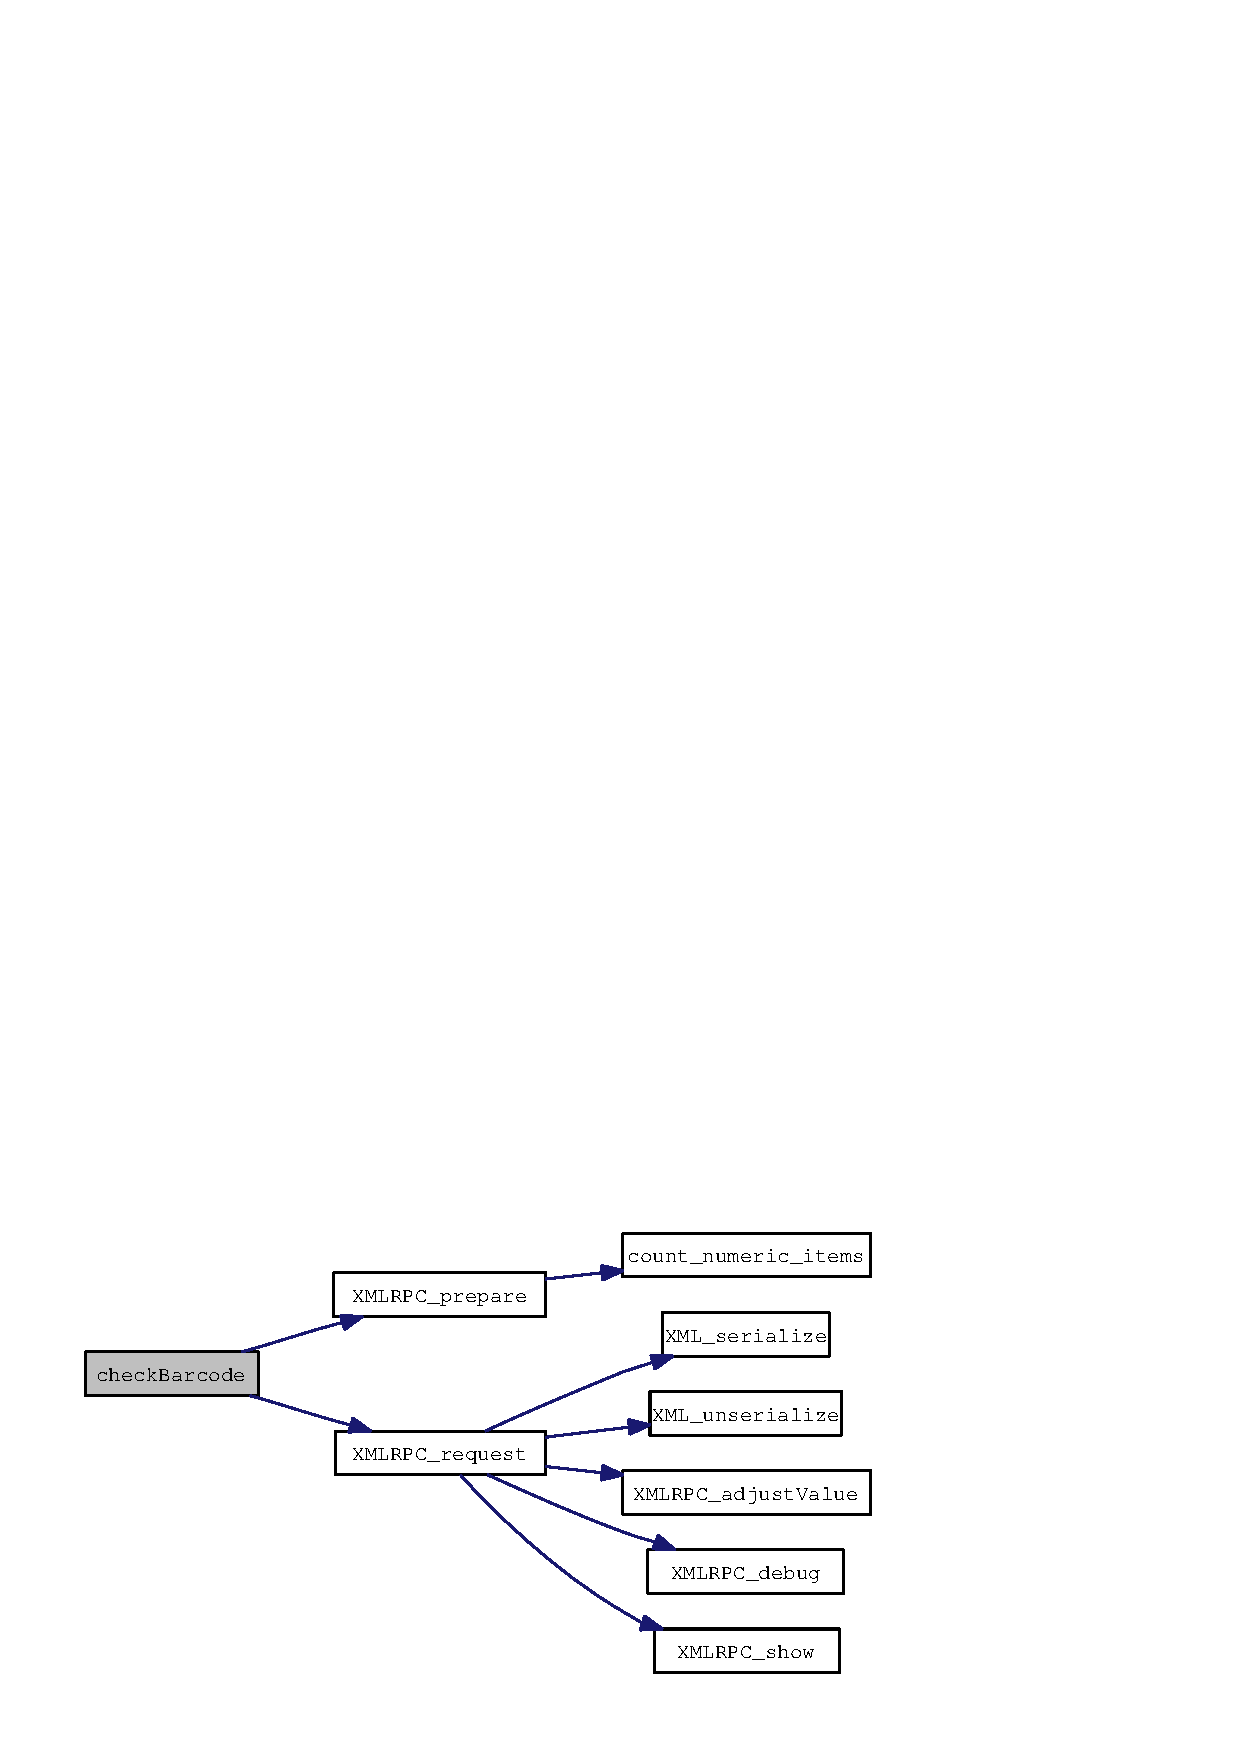
\includegraphics[width=211pt]{barcode_8inc_6d3645af0ef526e4f64d28dcbdceb74f_cgraph}
\end{center}
\end{figure}
\hypertarget{barcode_8inc_e10c37e4f9f9b7c6617a388351a27c99}{
\index{barcode.inc@{barcode.inc}!getBarcodeInfo@{getBarcodeInfo}}
\index{getBarcodeInfo@{getBarcodeInfo}!barcode.inc@{barcode.inc}}
\subsubsection{\setlength{\rightskip}{0pt plus 5cm}getBarcodeInfo (\$ {\em barcode})}}
\label{barcode_8inc_e10c37e4f9f9b7c6617a388351a27c99}


Output Barcode Info \begin{Desc}
\item[Parameters:]
\begin{description}
\item[{\em \$barcode}]The barcode to lookup \end{description}
\end{Desc}
\begin{Desc}
\item[Returns:]HTML code to create the info area \end{Desc}
\begin{Desc}
\item[See also:]\hyperlink{barcode_8inc_6d3645af0ef526e4f64d28dcbdceb74f}{checkBarcode} \end{Desc}


Hold the HTML code to be outputted

Array containinf info on the given UPC 

Definition at line 38 of file barcode.inc.

References XMLRPC\_\-prepare(), and XMLRPC\_\-request().

Here is the call graph for this function:\nopagebreak
\begin{figure}[H]
\begin{center}
\leavevmode
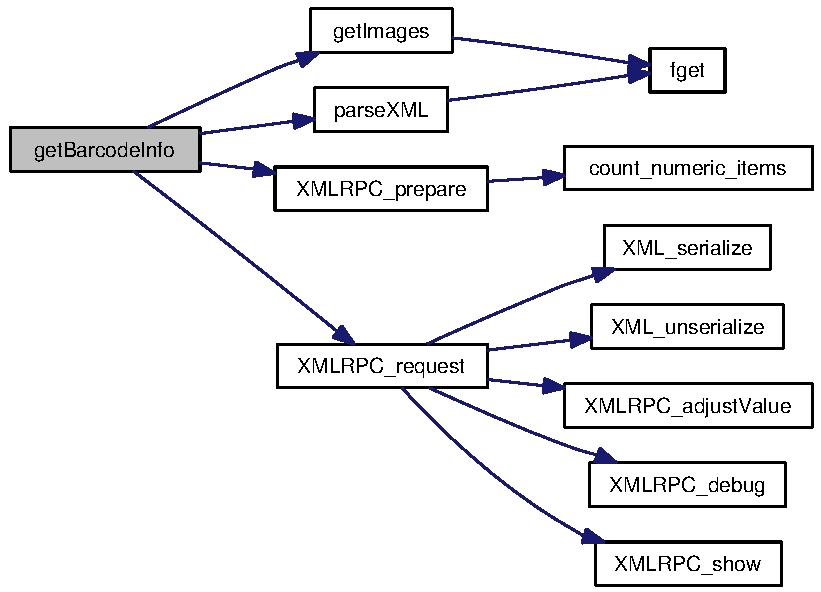
\includegraphics[width=215pt]{barcode_8inc_e10c37e4f9f9b7c6617a388351a27c99_cgraph}
\end{center}
\end{figure}
